%%%%%%%%%%%%%%%%%%%%%%%%%%%%%%%%%%%%%%%%%%%%%%%%%%%%%%%%%%%%%%%%%%%%%%%%%%%%%%%%
%%%%%%%%%%%%%%%%%%%%%%%%%%%%%%%%%%%%%%%%%%%%%%%%%%%%%%%%%%%%%%%%%%%%%%%%%%%%%%%%
%
% A general frame for lecture slides and lecture notes in one file
% using LaTeX beamer
%
%%%%%%%%%%%%%%%%%%%%%%%%%%%%%%%%%%%%%%%%%%%%%%%%%%%%%%%%%%%%%%%%%%%%%%%%%%%%%%%%
%%%%%%%%%%%%%%%%%%%%%%%%%%%%%%%%%%%%%%%%%%%%%%%%%%%%%%%%%%%%%%%%%%%%%%%%%%%%%%%%
\documentclass[11pt]{beamer}
%\usepackage[ngerman]{babel}
\usepackage[T1]{fontenc}
\usepackage[utf8]{inputenc}
\usepackage{lmodern}
\usepackage{tcolorbox}
\usepackage{amsmath,amssymb,amsfonts}


% only presentation
\mode<presentation>
{
  \usetheme{default}
%  \usecolortheme{crane}
  \setbeamercovered{transparent}
%  \setlength{\parindent}{0pt}
%  \setlength{\parskip}{1.35ex plus 0.5ex minus 0.3ex}
%  \usefonttheme{structuresmallcapsserif}
  \usefonttheme{structurebold}
  \setbeamertemplate{theorems}[numbered]
  \setbeamertemplate{sidebar right}{}
  \usepackage{amscd}
}

% all after
\usepackage{tikz}
\usepackage{pgfplots,adjustbox}
\usepackage{eurosym}
\usepackage{graphicx}
\graphicspath{{.}{figures/}}
\usepackage{multimedia}
\usepackage{psfrag}
\usepackage{listings}
% \lstset{language=C++, basicstyle=\ttfamily,
%   keywordstyle=\color{black}\bfseries, tabsize=4, stringstyle=\ttfamily,
%   commentstyle=\it, extendedchars=true, escapeinside={/*@}{@*/}}
\lstset{language=C++, basicstyle=\small\ttfamily,
  keywordstyle=\bfseries, tabsize=4, stringstyle=\ttfamily,morekeywords={decltype},
  extendedchars=true, escapeinside={/*@}{@*/}}
\definecolor{darkgray}{gray}{0.4}
\lstset{keywordstyle=\color{green!40!black},
  commentstyle=\itshape\color{blue!30!black!40!white},
  stringstyle=\color{blue!60!black!60!white},
  emph={bool,int,unsigned,char,true,false,void}, emphstyle=\color{red!80!black},
  emph={[2]\#include,\#define,\#ifdef,\#endif}, emphstyle={[2]\color{green!60!black}},
  emph={[3]Dune,Grid,SomeGrid,TheGrid,LeafIterator,LevelIterator,LeafIntersectionIterator,LevelIntersectionIterator,Geometry,GeometryType,QuadraturePoint,QuadratureRule,PDELab,Entity,EntityPointer,Codim,FieldVector,FieldMatrix}, emphstyle={[3]\color{blue!60!black}}
}
\usepackage{curves}
%\usepackage{epic}
\usepackage{calc}
%\usepackage{picinpar}
%\usepackage{fancybox}
%\usepackage{xspace}
\usepackage{enumerate}
\usepackage{algpseudocode}
\usepackage{color}
\usepackage{bold-extra}
\usepackage{bm}
\usepackage{stmaryrd}
%\usepackage[squaren]{SIunits}
\usepackage{nicefrac}

\usepackage{fancyvrb,bbm,xspace}
\usepackage{lmodern}
\usepackage{fancyvrb,bbm,xspace}
\usepackage[binary-units]{siunitx}
\usepackage{xcolor,tabu}

\usepackage{svg}

\definecolor{niceblue}{rgb}{0.122,0.396,0.651}   %% 31, 101, 166 or #1F65A6
\definecolor{niceorange}{RGB}{255,205,86}        %% #FFCD56
\definecolor{nicered}{RGB}{220,20,60}                      %% rgb(220, 20, 60)
\definecolor{niceteal}{HTML}{00A9AB}
\definecolor{niceviolet}{HTML}{820080}

\def\clap#1{\hbox to 0pt{\hss#1\hss}}
\definecolor{dunedarkblue}{rgb}{0.22, 0.29, 0.49}
\definecolor{dunemediumblue}{rgb}{0.35, 0.45, 0.71}
\definecolor{dunelightblue}{rgb}{0.61, 0.68, 0.85}
\definecolor{duneorange}{rgb}{0.91, 0.56, 0.25}

\definecolor{niceblueLight}{HTML}{91CAFB}
\definecolor{niceblueVeryLight}{HTML}{DDEFFF}

\usepackage{lmodern}
\usepackage{inconsolata}
\usepackage{nimbusmononarrow}
%\renewcommand*\ttdefault{txtt}
\usepackage{dsfont}

\mode<presentation>
{
\theoremstyle{definition}
\setbeamertemplate{footline}[frame number]
}
% \newtheorem{Def}{Definition}%[section]
% \newtheorem{Exm}[Def]{Example}
% \newtheorem{Lem}[Def]{Lemma}
% \newtheorem{Rem}[Def]{Remark}
% \newtheorem{Rul}[Def]{Rule}
% \newtheorem{Thm}[Def]{Theorem}
% \newtheorem{Cor}[Def]{Corollary}
% \newtheorem{Obs}[Def]{Observation}
% \newtheorem{Ass}[Def]{Assumption}
% \newtheorem{Pro}[Def]{Property}
% \newtheorem{Alg}[Def]{Algorithm}
% \newtheorem{Prp}[Def]{Proposition}
% \newtheorem{Lst}[Def]{Listing}

\newenvironment{codeblock}{%
  \begin{tcolorbox}[size=small,oversize,boxrule=0pt,opacityframe=0,colback=blue!30!black!5!white]}{%
  \end{tcolorbox}}
\usepackage{verbatim}
\makeatletter
\newwrite\lstvrb@out
\newenvironment{cppcode}{%
  \begingroup
  \@bsphack
  \immediate\openout\lstvrb@out\jobname.lst
  \let\do\@makeother\dospecials\catcode`\^^M\active
  \def\verbatim@processline{%
    \immediate\write\lstvrb@out{\the\verbatim@line}}%
  \verbatim@start}{%
  \immediate\closeout\lstvrb@out
  \@esphack
  \endgroup
  \begin{codeblock}
    \vspace*{-1ex}
    \lstinputlisting[basicstyle=\scriptsize\ttfamily]{\jobname.lst}
    \vspace*{-1ex}
  \end{codeblock}}
\makeatother
\newcommand{\rightarrownice}{\tikz{%
    \draw[-latex,line width=2pt, color=structure.fg]   (0pt,0pt) -- +(2em,0) node[thin,right] {};}}

% math symbols
\newcommand{\C}{\mathbb{C}}
\newcommand{\R}{\mathbb{R}}
\newcommand{\N}{\mathbb{N}}
\newcommand{\Z}{\mathbb{Z}}
\newcommand{\Q}{\mathbb{Q}}
\newcommand{\K}{\mathbb{K}}
\newcommand{\blue}{\color[rgb]{0,0,1}}
\newcommand{\green}{\color[rgb]{0,1,0}}
\newcommand{\red}{\color[rgb]{1,0,0}}
\newcommand{\violet}{\color[rgb]{1,0,1}}
\newcommand{\uu}{\mathbf{u}}
\newcommand{\nn}{\mathbf{n}}
\newcommand{\diffd}{\,d}

% Delete this, if you do not want the table of contents to pop up at
% the beginning of each subsection:
\AtBeginSection[]
{
  \begin{frame}<beamer>
    \frametitle{Contents}
    \tableofcontents[sectionstyle=show/shaded,subsectionstyle=hide/hide/hide]
%\tableofcontents[currentsection]
  \end{frame}
}

% Title definition
\title{The DUNE Grid Interface\\An Introduction}
\author{Christian Engwer}
\institute[]
{
  Applied Mathematics, WWU Münster\\
  Orleans-Ring 10, 48149 Münster
}
\date{~}%March 7, 2017}

%%%%%%%%%%%%%%%%%%%%%%%%%%%%%%%%%%%%%%%%%%%%%%%%%%%%%%%%%%%%%%%%%%%%%%%%%%%%%%%%
%%%%%%%%%%%%%%%%%%%%%%%%%%%%%%%%%%%%%%%%%%%%%%%%%%%%%%%%%%%%%%%%%%%%%%%%%%%%%%%%
%
% now comes the individual stuff lecture by lecture
%
%%%%%%%%%%%%%%%%%%%%%%%%%%%%%%%%%%%%%%%%%%%%%%%%%%%%%%%%%%%%%%%%%%%%%%%%%%%%%%%%
%%%%%%%%%%%%%%%%%%%%%%%%%%%%%%%%%%%%%%%%%%%%%%%%%%%%%%%%%%%%%%%%%%%%%%%%%%%%%%%%

\begin{document}

\begin{frame}
    \titlepage
\end{frame}

\part{Dune Course: Design Principles}

\begin{onlyenv}<presentation>
\begin{frame}
   \partpage
   \pause
  \vfill
  \begin{quote}
    {\normalfont{}[...]} a modular toolbox for solving partial
    differential equations (PDEs) with grid-based
    methods {\normalfont{}[...]}

    \hfill--- {\normalfont \url{http://www.dune-project.org/}}
  \end{quote}
 \end{frame}
\end{onlyenv}

\section{Design Principles}

\begin{onlyenv}<presentation>
  \begin{frame} \frametitle{Design Principles}

    \begin{description}[Legacy Code:]
    \item[Flexibility:]
      {Seperation of data structures and algorithms.}\\[2ex]
    \item[Efficiency:]
      {Generic programming techniques.}\\[2ex]
    \item[Legacy Code:]
      {Reuse existing finite element software.}\\[2ex]
    \end{description}

  \end{frame}
\end{onlyenv}

\begin{frame} \frametitle{Flexibility}

  \framesubtitle<presentation>{Seperate data structures and algorithms.}

  \only<article>{Seperation of data structures and algorithms:}

  \begin{itemize}
  \item The algorithm determins the data structure to
    operate on.
  \item Data structures are hidden under a common interface.
  \item Algorithms work only on that interface.
  \item Different implementations of the interface.
  \end{itemize} \centerline{\includegraphics[width=0.8\textwidth]{abstractalgorithm}}
  \medskip
  \centerline{\includegraphics[width=0.8\textwidth]{abstractmatvec}}
\end{frame}

\begin{frame}
  \frametitle{Efficiency}

  \framesubtitle<presentation>{Implementation with generic programming
    techniques.}

  \only<article>{Generic programming techniques:}

  \begin{minipage}{0.35\textwidth}
    \begin{center}
      \includegraphics[width={\textwidth}]{generic}
    \end{center}
  \end{minipage}
  \begin{minipage}{0.65\textwidth-1ex}
    % \begin{itemize}
    % \item Static Polymorphism $\rightarrow$
    %   Compile-time selection of data structures.
    % \item Compiler generates code for each
    %   \mbox{(algorithm,data structure)} combination.
    % \item Allows interfaces with fine granularity.
    % \item All optimizations apply, in particular function inlining.
    % \item see i.e. STL, Blitz++, MTL,\ldots{}
    % \item and Thesis of Gundram Berti (2000): Concepts for grid based algorithms.
    % \end{itemize}
      \begin{enumerate}
      \item Static Polymorphism
        \begin{itemize}
        \item Duck Typing (see STL)
        \item Curiously Recurring Template Pattern (Barton and Nackman)
        \end{itemize}
      \item Grid Entity Ranges
        \begin{itemize}
        \item Generic access to different data structures.
        \end{itemize}
      \item View Concept
        \begin{itemize}
        \item Access to different partitions of one data set.
        \end{itemize}
      \end{enumerate}
  \end{minipage}
\end{frame}

\section{The DUNE Framework}

\begin{frame} \frametitle{The DUNE Framework}
  \label{dunedevelopment}
  \hspace*{-.7cm}
    \begin{minipage}[t]{0.54\textwidth}
        \begin{itemize}
        \item Modules
          \begin{onlyenv}<1>
            \begin{itemize}
            \item Code is split into separate modules.
            \item Applications use only the modules they need.
            \item Modules are sorted according to level of maturaty.
            \item Everybody can provide her/his own modules.
            \end{itemize}
          \end{onlyenv}
        \item Portability
          % \begin{onlyenv}<2>
          %   \begin{itemize}
          %   \item stick to the C++ standard
          %   \item use a portable tool chain
          %   \end{itemize}
          % \end{onlyenv}
        \item Open Development Process
          % \begin{onlyenv}<3>
          %   \begin{itemize}
          %   \item everybody can participate
          %   \item not bound to a set of research groups
          %   \end{itemize}
          % \end{onlyenv}
        \item Free Software Licence
          % \begin{onlyenv}<4>
          %   \begin{itemize}
          %   \item derived work must be published under the same
          %     license
          %   \item proprietary code can be built upon DUNE
          %   \end{itemize}
          % \end{onlyenv}
        \end{itemize}
    \end{minipage}
  \hspace*{.4cm}
    \begin{minipage}[t]{0.45\textwidth}
      \mbox{}
      \begin{center}
        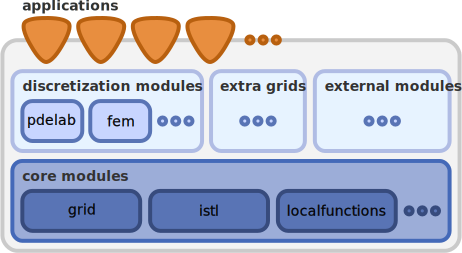
\includegraphics[width=\linewidth]{dunedesign}\\
        % {  \footnotesize \hfill [Bastian et. al. 2008:1, 2008:2]}\\[1cm]
        \scriptsize [Bastian,
        Blatt, Dedner, Engwer, Kl{\"{o}}fkorn, Kornhuber,
        Ohlberger, Sander 2008]
      \end{center}
    \end{minipage}
\end{frame}

\begin{frame}
  \frametitle{Some historic remarks}
  \centering
%  \includesvg[width=0.9\linewidth]{dunetimeline}
  \includegraphics[width=1.0\linewidth]{dunetimeline}
\end{frame}

\begin{frame} \frametitle{DUNE Release 2.6.0}
  % Upcoming stable version is 2.6.0,
  % \only<presentation>{  \\ \scriptsize
  %   \hspace*{4mm}}
  % currently available as release candidate.
  \footnotesize
  \begin{columns}[t]
    \begin{column}{0.5\textwidth}
\mode<presentation>{
      \begin{description}[dune-]
}
\mode<article>{
      \begin{description}[dune-localfunctions:]
}
      \item[dune-common:]
        foundation classes, infrastructure\mode<presentation>{\\[3ex]}
      \item[dune-geometry:]
        geometric mappings,\mode<presentation>{\\}
        quadrature rules
        visualization\mode<presentation>{\\[3ex]}
      \item[dune-grid:]
        grid interface,\mode<presentation>{\\}
        visualization
\mode<presentation>{
      \end{description}
    \end{column}
    \begin{column}{0.5\textwidth}
      \begin{description}[dune-]
}
      \item[dune-istl:]
        \emph{(Iterative Solver Template Library)}\\
        generic sparse matrix/vector classes,\\
        solvers (Krylov methods, AMG, etc.)
      \item[dune-localfunctions:]
        generic interface for local finite element
        functions. Abstract definition following Ciarlet.
        Collection of different finite elements.
      \end{description}
    \end{column}
  \end{columns}
  % \vfill
  % \vfill
  \mode<presentation>{
  \vspace*{4mm}
  \hspace*{0.5\linewidth}\clap{\fbox{\includegraphics[width=\linewidth]{dunebg}}}
  \hspace*{-0.5\linewidth}
  % \hspace*{1mm}
  \color{duneorange}
  \hspace*{2mm}
  \raisebox{2.5mm}{\bf \LARGE DUNE}\hspace*{5mm}
  \raisebox{3.5mm}{\large\href{http://www.dune-project.org/}{\texttt{\textbf{http://www.dune-project.org/}}}}
  }
\end{frame}

\only<article>{\enlargethispage{4ex}}

\begin{frame}[t] \frametitle{DUN(E)iverse}

  \hfill
\includegraphics[height=0.21\linewidth]{brick}
  \vspace*{-0.21\linewidth}
  \small
  \begin{itemize}
  \item modular structure
  \item write your own DUNE modules
  \item available under different licenses
  \end{itemize}
  \pause
  \begin{itemize}
  \item \structure{Discretization Modules}
    \begin{onlyenv}<2-3>
      \scriptsize
      \begin{description}[dune-networkgrid:]
        % \item[dune-disc:] shapefunctions, discretization schemes, \dots
      \item[\alert<3>{dune-pdelab:}]
        {Discretization module based on dune-localfunctions.}
      \item[dune-fem:] Discretization module based on dune-localfunctions.
      \item[dune-functions:] A new initiative to provide unified
        interfaces for functions and function spaces.
      \end{description}
    \end{onlyenv}
    \item \structure{Additional Grid Implementations}
      \begin{onlyenv}<4>
      \scriptsize
        \begin{description}[dune-networkgrid:]
        \item[dune-grid-glue:] allows to compute overlapping and
          nonoverlapping couplings of Dune grids, as required for most
          domain decomposition algorithms.
        \item[dune-subgrid:] allows you to work on a subset of a given DUNE
          grid.
        \item[dune-foamgrid:] non-manifold grids of 1d or 2d entities
          in higher-dimensional world.
        \item[dune-prismgrid:] is a tensorgrid of a 2D simplex grid and a
          1D grid.
        \item[dune-cornerpoint:] a cornerpoint mesh, compatible with the
          grid format of the ECLIPSE reservoir simulation software.\\[-3ex]
        \item[\large$\cdots$]
        \end{description}
      \end{onlyenv}
    \item \structure{Extension Modules}
      \begin{onlyenv}<5>
      \scriptsize
        \begin{description}[dune-networkgrid:]
          % \item[Kaskade 7:] Simulation Suite -- uses Dune for the grid and linear algebra infrastructure.
          % \item[DuMu$^{\text{x}}$:] simulations of flow and
          %   transport processes in porous media. Development is in an early
          %   state.
        \item[dune-python] python bindings for centrral DUNE components
        \item[dune-typetree] classes to organise types in trees
        \item[dune-dpg] construct optimal Discontinuous-Petrov-Galerkin test spaces
        \item[dune-tpmc] cut-cell construction using level-sets
        \item[\large$\cdots$]
        \end{description}
      \end{onlyenv}
    \end{itemize}
    \begin{onlyenv}<6>
      \small
      \begin{itemize}
      \item[Goals:] allow people to\ldots{}\scriptsize
        \begin{itemize}
        \item get credit for their innvoations
        \item experiment without breaking the core
        \item develop at different speeds
        \end{itemize}
    \end{itemize}
    \end{onlyenv}
\end{frame}

\newcommand{\cmd}[1]{\structure{\texttt{\normalsize #1}}}
\begin{frame}
  \frametitle{A Package System}

  \vspace*{-1ex}
  \small
  \begin{columns}
    \begin{column}{0.65\linewidth}
    \cmd{\Large dunecontrol}
      \begin{itemize}
      \item control of module-interplay
      \item suggestions \& dependencies
      \item intergrates with cmake \& git
      \item works with Linux, Mac and Mingw
      \end{itemize}
    \end{column}
    \begin{column}{0.3\linewidth}
%      \includesvg[width=\linewidth]{Gnome-emblem-package}\\\centering
      
\includegraphics[width=\linewidth]{Gnome-emblem-package}\\\centering
      \tiny Source: gnome
    \end{column}
  \end{columns}

  \pause
  \structure{Note:} Dependencies should form a DAG

  \pause
  \medskip
  \cmd{dunecontrol cmake}\\\qquad
  configure packages via cmake, include necessary path information\\
  \cmd{dunecontrol make}\\\qquad
  build packages in correct order

  \medskip
  \structure{\ldots{}} works without \cmd{make install}

\end{frame}

% \begin{frame} \frametitle{DUNE ecosystem}
%   \begin{itemize}
%     \only<presentation>{\footnotesize}
%   \item modular structure
%   \item write your own DUNE modules
%   \item available under different licenses
%   \end{itemize}
%   \only<presentation>{\scriptsize}
%   \pause
%   %\vfill
%   \structure{Discretization Modules:}
%   \begin{description}[dune-networkgrid:]
%   % \item[dune-disc:] shapefunctions, discretization schemes, \dots
%     \item[\only<3>{\alert}{dune-pdelab:}]
%       {discretization module based on dune-localfunctions.}
%     \item[dune-fem:] Alternative implementation of finite element functions.
%     \item[dune-functions:] A new initiative to provide unified
%       interfaces for functions and function spaces.
%   \end{description}
%   \pause
%   \pause
%   \structure{External Modules:}
%   \begin{description}[dune-networkgrid:]
%   % \item[dune-disc:] shapefunctions, discretization schemes, \dots
%     \item[Kaskade 7:] Simulation Suite -- uses Dune for the grid and linear algebra infrastructure.
%     \item[DuMu$^{\text{x}}$:] simulations of flow and
%       transport processes in porous media. Development is in an early
%       state.
%     \item[dune-grid-glue:] allows to compute overlapping and
%       nonoverlapping couplings of Dune grids, as required for most
%       domain decomposition algorithms.
%     \item[dune-subgrid:] allows you to work on a subset of a given DUNE
%       grid.
%     \item[dune-networkgrid:] is a grid manager for a network of 1d
%       entities in a 3d world.
%     \item[dune-prismgrid:] is a tensorgrid of a 2D simplex grid and a
%       1D grid.
%     \item[dune-cornerpoint:] a cornerpoint mesh, compatible with the
%       grid format of the ECLIPSE reservoir simulation software.
%     \item[\large$\cdots$]
%   \end{description}
% \end{frame}

\part{Dune Course: Grid Module}

\begin{frame}
  \partpage
  \vfill
  \begin{quote}
  People think that computer science is the art of geniuses but the
  actual reality is the opposite, just many people doing things that
  build on each other, like a wall of mini stones.

  \hfill--- Donald E. Knuth
  \end{quote}
\end{frame}

% \begin{frame}
%   \titlepage
%   \uncover<2->{
%   \begin{quote}
%     People think that computer science is the art of geniuses but the
%     actual reality is the opposite, just many people doing things that
%     build on each other, like a wall of mini stones.

%     \hfill--- Donald E. Knuth
%   \end{quote}}
% \end{frame}

\begin{frame}
  \frametitle{Why Grids?}
  Weak formulation of boundary value problem:\\
  \begin{equation*}
    \text{Find $u \in U$ s.t.}\qquad
    a(u,v) = l(v) \quad \forall\,v \in V.
  \end{equation*}
  $a(u,v)$ and $l(v)$ are (bi)linear forms, e.g.
  \begin{equation*}
    a(u,v) = \int_\Omega \nabla u \cdot \nabla v \diffd x,
  \end{equation*}
  \raisebox{2ex}{with spatial domain $\Omega \subset \R^d$.}

  \pause
Grids are necessary for at least three reasons:
  \begin{enumerate}
  \item Piecewise description of the complicated domain $\Omega$
  \item Piecewise approximation of functions (by polynomials)
  \item Piecewise computation of integrals (by numerical quadrature)
  \end{enumerate}
\end{frame}


\begin{frame}
  \frametitle{Numerical Quadrature}
  \begin{itemize}
  \item Approximate integral by a weighted sum of function evaluations at sampling points:
  \begin{equation*}
    \int_{\hat\Omega} f(x) \diffd x \approx \sum_{i = 1}^N w_i f(x_i)
  \end{equation*}
  with weights $w_i$ and sampling points $x_i$, $i = 1,\dots,N$.\\[1em]
\item Different construction methods for $w_i$ and $x_i$
  \begin{itemize}
  \item Typically uses series of polynomials (Legendre, Lagrange, Lobatto, \dots).
  \item Exact for polynomial $f$ up to a predefined order.
  \end{itemize}
\item Quadrature scheme depends on $\hat\Omega$!
  \begin{itemize}
  \item Most schemes only available for simple shapes (triangle, square, tetrahedron, \dots).
  \item Quadrature on complicated shapes done by approximating $\Omega$ by small volumes of regular shape.
  \end{itemize}
  \end{itemize}
\end{frame}


\begin{frame}
  \frametitle{Computational Grid}
  \begin{columns}
    \begin{column}{0.3\textwidth}
      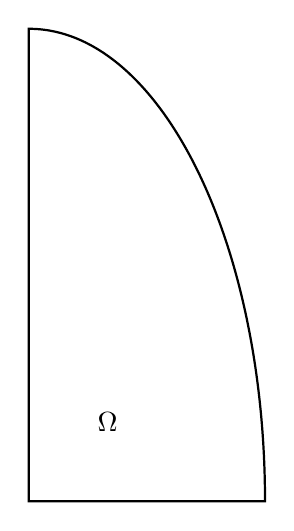
\begin{tikzpicture}
        \draw[thick]
        (0,0) -- (3,0) arc[start angle=0, end angle=90, x radius=3, y radius=6] -- cycle;
        \node at (1,1) {$\Omega$};
      \end{tikzpicture}
    \end{column}
    \begin{column}{0.3\textwidth}
      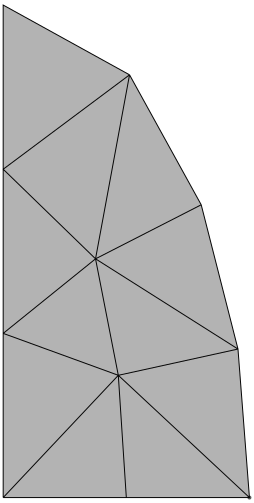
\includegraphics[width=3cm]{ellipsemeshcoarse-cropped}
    \end{column}
    \begin{column}{0.3\textwidth}
      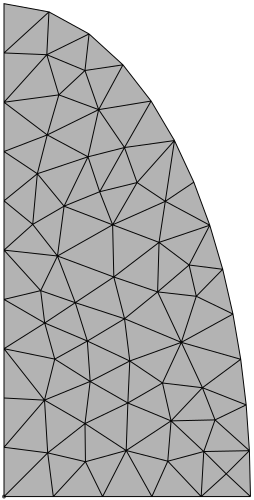
\includegraphics[width=3cm]{ellipsemesh-cropped}
    \end{column}
  \end{columns}
\end{frame}

\begin{frame} \frametitle{The DUNE Grid Module}
  \begin{itemize}
  \item The DUNE Grid Module is one of the five DUNE Core Modules.

  \item DUNE wants to provide an interfaces for grid-based
    methods. Therefore the concept of a \emph{Grid} is the central part
    of DUNE.

  \item \texttt{dune-grid} provides the interfaces, following the concept
    of a \emph{Grid}.

  \item Its implementation follows the three \emph{design principles} of
    DUNE:
    \begin{description}[~~~Legacy Code:]
    \item[Flexibility:]
      \onslide<0->{Separation of data structures and algorithms.}
    \item[Efficiency:]
      \onslide<0->{Generic programming techniques.}
    \item[Legacy Code:]
      \onslide<0->{Reuse existing finite element software.}
    \end{description}

  \end{itemize}
\end{frame}

\begin{frame}
  \frametitle<presentation>{Designed to support a wide range of Grids}
  \includegraphics[width=\linewidth]{grids}
\end{frame}

\begin{frame}
\frametitle{DUNE Grid Interface\footnote{\tiny Bastian,
Blatt, Dedner, Engwer, Kl{\"{o}}fkorn, Kornhuber,
Ohlberger, Sander: {\em A generic grid interface for parallel and adaptive
  scientific computing. Part {I}: Implementation and tests in {DUNE}}.
  Computing, 82(2-3):121--138, 2008.} Features}
\begin{itemize}
\item Provide abstract interface to grids with:
\begin{itemize}
\item Arbitrary dimension embedded in a world dimension,
\item multiple element types,
\item conforming or nonconforming,
\item hierarchical, local refinement,
\item arbitrary refinement rules (conforming or nonconforming),
\item parallel data distribution and communication,
\item dynamic load balancing.
\end{itemize}
\item Reuse existing implementations (ALU, UG, Alberta) + special
implementations (YaspGrid, FoamGrid).
\item Meta-Grids built on-top of the interface (GeometryGrid, SubGrid,
  MultiDomainGrid)
\end{itemize}
\end{frame}

\section{The Grid}

\begin{frame}
  \frametitle{The Grid}
  \emph{A formal specification of grids is required to enable an
  accurate description of the grid interface.}
  \only<presentation>{\vspace*{5mm}}
  \begin{columns}
    \begin{column}{0.33\linewidth}
      \only<presentation>{
      \includegraphics[width=0.9\linewidth]{hierref}\\
      \centerline{\tiny Hierarchic Grid}}
    \end{column}\hfill
    \begin{column}{0.6\linewidth}
      In DUNE a \emph{Grid} is always a hierarchic grid of dimension
      $d$, existing in a $w$ dimensional
      space. \only<presentation>{\par}
      The Grid is parametrised by
      \begin{itemize}
      \item the dimension $d$,
      \item the world dimension $w$
      \item and the maximum level $J$.
      \end{itemize}
    \end{column}
  \end{columns}
  \pause
  \vspace*{5mm}
  \emph{Within todays excercises we will always assume $d=w$ and we will
    ignore the hierarchic structure of the grids we deal with.}
\end{frame}

\begin{frame} \frametitle{The Grid\ldots A Container of Entities\ldots}

  \setbeamertemplate{itemize/enumerate body begin}{\setlength{\leftmargini}{0pt}}

  In the DUNE sense a \emph{Grid} is a container of entities:

  \medskip
  \begin{overlayarea}{\linewidth}{0.4\textheight}
    \begin{columns}
      \begin{column}{5mm}
      \end{column}
      \begin{column}{0.5\linewidth-3mm}
        \includegraphics<1-2>[width=1\linewidth]{entities}
        \includegraphics<3->[width=1\linewidth]{entities_cd}
      \end{column}\hfill
      \begin{column}{0.5\linewidth}
        \begin{itemize}
        \item vertices \only<3->{\emph{(Entity codim = $d$)}},
        \item edges \only<3->{\emph{(Entity codim = $d-1$)}},
        \item faces \only<3->{\emph{(Entity codim = $1$)}},
        \item cells \only<3->{\emph{(Entity codim = $0$)}}, \ldots{}
        \end{itemize}
      \end{column}
    \end{columns}
  \end{overlayarea}
  \pause{In order to do dimension independent programming, we need a
    dimension independent naming for different entities.}
  \only<presentation>{\par}
  \pause{We distinguish entities according to their codimension.}
  \only<presentation>{\par}
  Entities of codim = $c$ contain subentities of codim = $c+1$. This
  gives a recursive construction down to codim = $d$.

\end{frame}

\begin{frame}[fragile,fragile] \frametitle{The DUNE Grid Interface}
  The DUNE Grid Interface is a collection of classes and methods

  \only<presentation>{\vfill}
\begin{cppcode}
#include <dune/grid/yaspgrid.hh>

...

using Grid = Dune::YaspGrid<2>;
Grid grid({4,4},{1.0,1.0},{false,false});
auto gv = grid.leafGridView();
for (const auto& cell : elements(gv)) {
  // do something
}
\end{cppcode}

  \only<presentation>{\vfill}

  \pause
  \only<presentation>{\vfill}
  \emph{We will now get to know the most important classes and see how they
  interact.}
\end{frame}

\begin{frame} \frametitle{Modifying a Grid}
  The DUNE Grid interface follows the \emph{View-only} Concept.
  \pause
  \only<presentation>{\vfill}
  \structure{View-Only Concept}
  \begin{itemize}
  \item Views offer (read-only) access to the data
    \begin{itemize}
    \item Read-only access to grid entities allow the consequent use of
      \lstinline!const!.
    \item Access to entities is only through iterators for a
      certain view.
      \begin{itemize}
      \item[\rightarrownice] \emph{This allows on-the-fly implementations.}
      \end{itemize}
    \end{itemize}
  \item  Data can only be modified in the primary container \emph{(the Grid)}
  \end{itemize}
  \pause
  \only<presentation>{\vfill}
  \structure{Modification Methods:}
  \begin{itemize}
  \item  Global Refinement

  \item  Local Refinement \& Adaption

  \item  Load Balancing
  \end{itemize}
\end{frame}

\section{Views to the Grid}

\begin{frame} \frametitle{Views to the Grid}

  A Grid offers two major views:

  \only<presentation>{\vspace*{5mm}}
  \begin{columns}
    \begin{column}{0.5\linewidth}
      \includegraphics<1-2>[width=\linewidth]{views}
      \includegraphics<3->[width=\linewidth]{views2}
    \end{column}
    \begin{column}{0.5\linewidth}
      \structure{levelwise:}\\
      \only<presentation>{\small}
      all entities associated with the same level.\\
      \uncover<2->{
        \emph{Note: not all levels must cover the whole domain.}}

      \only<presentation>{\vspace*{5mm}}
      \normalsize
      \structure{leafwise:}\\
      \only<presentation>{\small}
      all leaf entities (entities which are not refined).\\
      \uncover<3->{
        The leaf view can be seen as the projection of a
        levels onto a flat grid. It again covers the whole domain.}
    \end{column}
  \end{columns}

\end{frame}

\begin{frame} \frametitle{Views to the Grid}
  \framesubtitle{Dune::GridView}

  \begin{itemize}
  \item The \lstinline!Dune::GridView!  class consolidates all
    information depending on the current View.
    \pause
  \item Every Grid must provide
    \begin{itemize}
    \item \lstinline!Grid::LeafGridView! and
    \item \lstinline!Grid::LevelGridView!.
    \end{itemize}
    \pause

  \item The \lstinline!Grid! creates a new view every time you ask it for one, so you need
    to store a copy of it.
  \item Accessing the Views:
    \begin{itemize}
    \item \lstinline!Grid::leafGridView()! and
    \item \lstinline!Grid::levelGridView(int level)!.
    \end{itemize}
  \end{itemize}
\end{frame}

\begin{frame}[fragile]
  \frametitle{Iterating over grid entities}
Typically, most code uses the grid to iterate over some of its entities (e.g.\ cells) and perform
some calculations with each of those entities.
\begin{itemize}
\item \lstinline!GridView! supports iteration over all entities of one codimension.
\item Iteration uses C++11 range-based for loops:
  \begin{cppcode}
for (const auto& cell : elements(gv)) {
  // do some work with cell
}
  \end{cppcode}
\item The type in front of \lstinline!cell! is important:
  \begin{itemize}
  \item If you create an entity in a range-based for loop, use \lstinline!const auto&!.
  \item In \emph{all} other cases, use plain \lstinline!auto!!
  \end{itemize}
  If you do not follow this advice, your program may crash in unpredictable ways.
\end{itemize}
\end{frame}

\begin{frame}[fragile]
  \frametitle{Iteration functions}
  \begin{cppcode}
for (const auto& cell : elements(gv)) {
  // do some work with cell
}
  \end{cppcode}
  Depending on the entities you are interested in, you can use one of the following functions:
  \begin{cppcode}
// Iterates over cells   (codim = 0)
for (const auto& c : elements(gv))
// Iterates over vertices  (dim = 0)
for (const auto& v : vertices(gv))
// Iterates over facets  (codim = 1)
for (const auto& f : facets(gv))
// Iterates over edges     (dim = 1)
for (const auto& e : edges(gv))

// Iterates over entities with a given codimension (here: 2)
for (const auto& e : entities(gv,Dune::Codim<2>{}))
// Iterates over entities with a given dimension (here: 2)
for (const auto& e : entities(gv,Dune::Dim<2>{}))
  \end{cppcode}
\end{frame}

% \begin{frame}[fragile]
% \begin{center}
% Go to code example 1 \ldots
% \end{center}
% \end{frame}

% \begin{frame}
%   \frametitle{LevelGridView versus LeafGridView}
%   \begin{columns}
%     \begin{column}{0.47\linewidth}
%       \begin{center}
%         \begin{onlyenv}<article>
%           \includegraphics[width=0.7\linewidth]{iterators}
%         \end{onlyenv}
%       \end{center}
%       \begin{onlyenv}<presentation>
%         \includegraphics[width=\linewidth]{iterators}
%       \end{onlyenv}
%     \end{column}
%     \begin{column}{0.53\linewidth}
%     \end{column}
%   \end{columns}
% \end{frame}


\section{Entities}

\begin{frame}[fragile] \frametitle{Entities}

  \structure{Iterating over a grid view, we get access to the entities.}

  \begin{cppcode}
for (const auto& cell : elements(gv)) {
  cell.?????(); // what can we do here?
}
  \end{cppcode}

  \pause
  \begin{itemize}
  \item Entities cannot be modified.
  \item Entities can be copied and stored\\(but copies might be expensive!).
    \pause
  \item Entities provide topological and geometrical information.
  \end{itemize}
\end{frame}

\begin{frame}
  \frametitle{Entities}

  \structure{An Entity $E$ provides both topological information}
  \begin{itemize}
  \item Type of the entity (triangle, quadrilateral, etc.).
  \item Relations to other entities.
  \end{itemize}
  \structure{and geometrical information}
  \begin{itemize}
  \item Position of the entity in the grid.
  \end{itemize}

  \only<presentation>{\vfill}
  \pause
  \begin{columns}
    \begin{column}{5mm}
    \end{column}
    \begin{column}{0.4\textwidth}
      \begin{center}
        \visible<presentation|2->{
          \includegraphics[width=\linewidth]{refelem-mapping}}\\
        \begin{onlyenv}<article>
          \includegraphics[width=0.6\linewidth]{refelem-mapping}\\
        \end{onlyenv}
        \centerline{\tiny Mapping from $\hat{\Omega}$ into global coordinates.}
      \end{center}
    \end{column}
    \begin{column}{0.5\textwidth}
      \structure{Entity $E$ is defined by\dots{}}
        \begin{itemize}
        \item Reference Element $\hat{\Omega}$
        \item Transformation $T_E$
        \end{itemize}
    \end{column}
  \end{columns}

  \only<presentation>{\vfill}
  \pause
  \lstinline!GridView::Codim<c>::Entity!
  implements the entity concept.

\end{frame}

\begin{frame}[fragile]
  \frametitle{Dimension and Codimension}
  Each entity has a \structure{dimension}:
  \begin{columns}
    \begin{column}{0.5\textwidth}
      \begin{itemize}
      \item \lstinline!dim(vertex) == 0!
      \item \lstinline!dim(line) == 1!
      \end{itemize}
    \end{column}
    \begin{column}{0.5\textwidth}
      \begin{itemize}
      \item \lstinline!dim(triangle) == 2!
      \item \dots
      \end{itemize}
    \end{column}
    \end{columns}
  \pause\vspace*{2em}
  When writing dimension-independent code, it is often easier to instead use the \structure{codimension}.\\[1em]
  The codimension of an entity $e$ is always relative to the dimension of the grid and is given by:
  \begin{equation*}
    \mathrm{codim}(e) = \mathrm{dim}(grid) - \mathrm{dim}(e)
  \end{equation*}
  \begin{columns}
    \begin{column}{0.5\textwidth}
      \begin{itemize}
      \item \lstinline!codim(cell) == 0!
      \item \lstinline!codim(face) == 1!
      \end{itemize}
    \end{column}
    \begin{column}{0.5\textwidth}
      \begin{itemize}
      \item \dots
      \item \lstinline!codim(vertex) == dim(grid)!
      \end{itemize}
    \end{column}
    \end{columns}

\end{frame}

\begin{frame}[fragile]
  \frametitle{Storing Entities}

  \vfill

  \pause
  \lstinline!GridView::Codim<c>::Entity!
  \begin{itemize}
  \item Entities can be copied and stored like any normal object.
  \item Important: There can be \emph{multiple} entity objects for a single logical grid entity (because they can be copied)
  \item \emph{Memory expensive, but fast.}
  \end{itemize}

  \vfill

  \pause

  \lstinline!GridView::Codim<c>::EntitySeed!


  \begin{itemize}
  \item Store minimal information to find an entity again.
  \item Create like this:
    \begin{cppcode}
auto entity_seed = entity.seed();
    \end{cppcode}
  \item The grid can create a new \lstinline!Entity! object from an \lstinline!EntitySeed!:
    \begin{cppcode}
auto entity = grid.entity(entity_seed);
    \end{cppcode}
  \item \emph{Memory efficient, but run-time overhead to recreate entity.}
  \end{itemize}

\end{frame}

% \only<article>{\newpage}

\subsection{Reference Elements}
\begin{frame}[fragile] \frametitle{Reference Elements}

  \begin{description}
  \item[\tt Dune::GeometryType] identifies the type of the
    entity's reference element.
  \item[\tt Grid::Codim<c>::Entity::type()]
    returns the \lstinline!GeometryType! of an entity.
  \end{description}

  \begin{onlyenv}<presentation>
    ~\hfill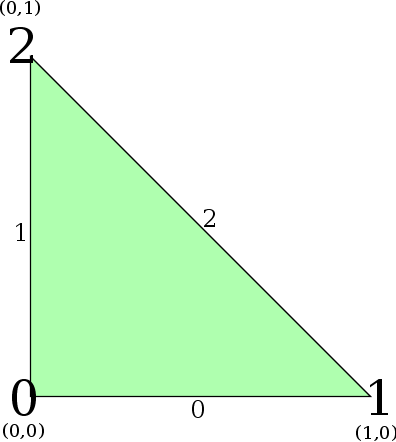
\includegraphics[width=0.24\linewidth]{gg_triangle}
    \hfill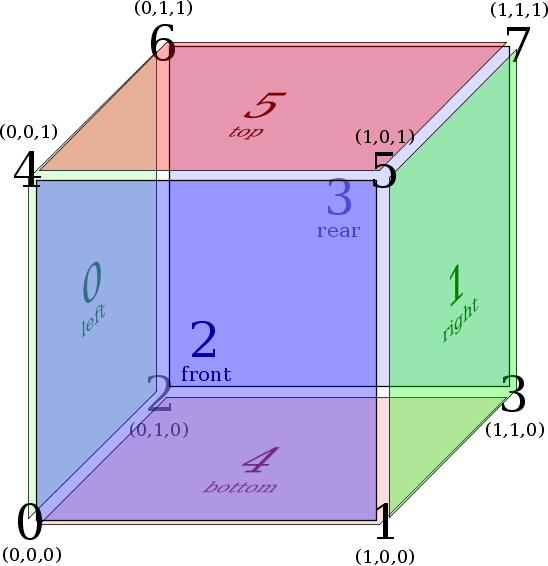
\includegraphics[width=0.28\linewidth]{gg_hexahedron}
    \hfill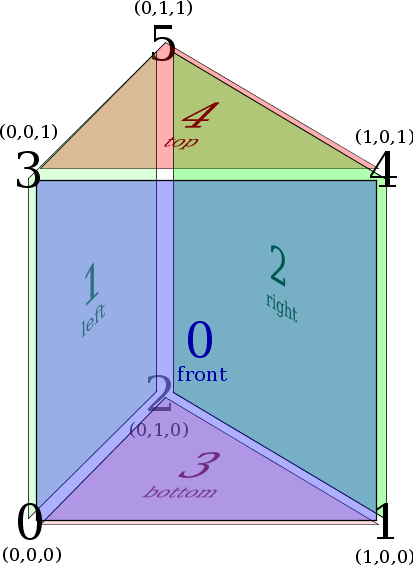
\includegraphics[width=0.22\linewidth]{gg_prism}
    \hfill~

    ~\hfill\parbox{0.24\linewidth}{\centering simplex 2D}
    \hfill\parbox{0.28\linewidth}{\centering cube 3D}
    \hfill\parbox{0.22\linewidth}{\centering prism} \hfill~
  \end{onlyenv}
  \begin{onlyenv}<article>
    \textbf{1D}:
    \begin{center}
      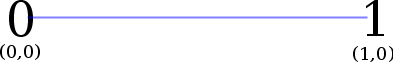
\includegraphics[width=0.23\linewidth]{gg_line}

      line 1D (both simplex 1D \& cube 1D)
    \end{center}
    \textbf{2D:}
    \begin{center}
      \begin{tabular}{cccc}
        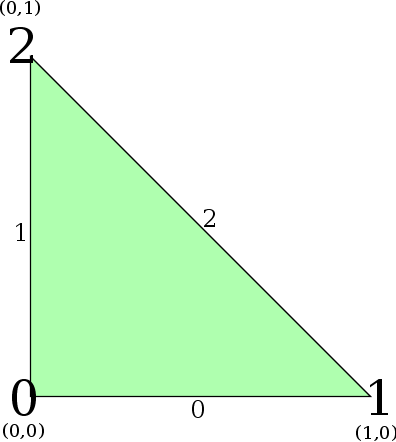
\includegraphics[height=0.23\linewidth]{gg_triangle} &
        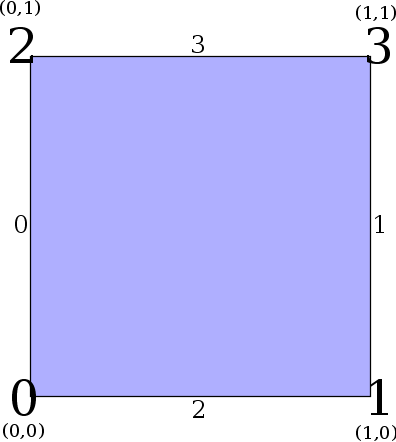
\includegraphics[height=0.23\linewidth]{gg_quadrilateral}\\
        simplex 2D & cube 2D\\
      \end{tabular}
    \end{center}
    \textbf{3D:}
    \begin{center}
      \begin{tabular}{cccc}
        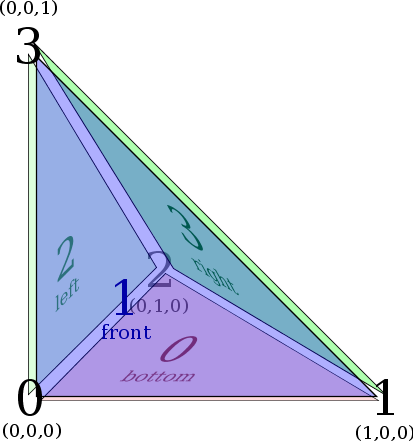
\includegraphics[height=0.23\linewidth]{gg_tetrahedron} &
        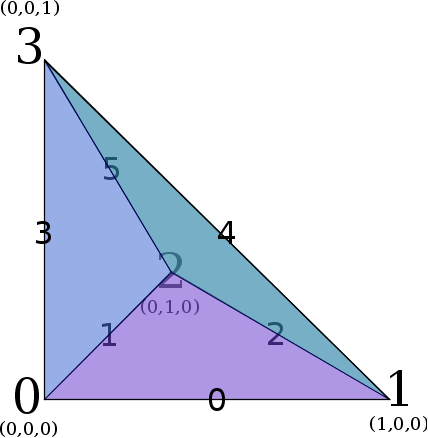
\includegraphics[height=0.23\linewidth]{gg_tetrahedron_edges} &
        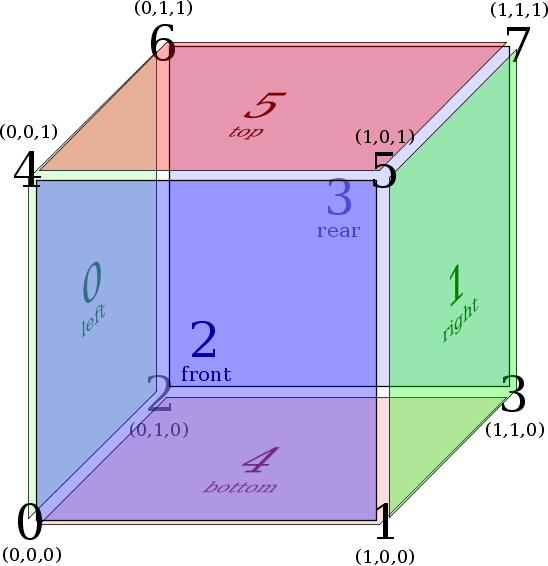
\includegraphics[height=0.23\linewidth]{gg_hexahedron} &
        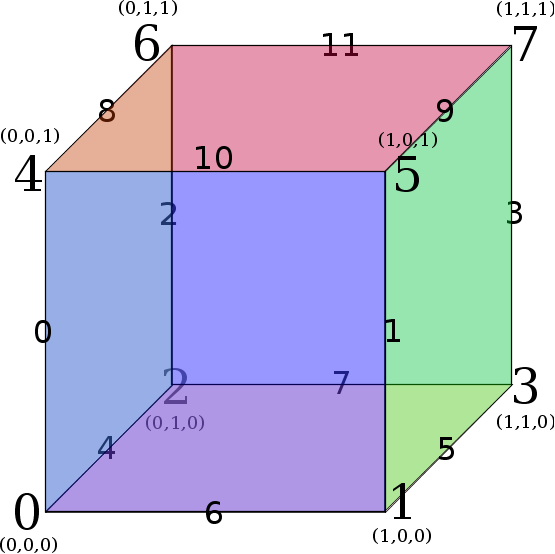
\includegraphics[height=0.23\linewidth]{gg_hexahedron_edges}
        \\
        simplex 3D (faces) & simplex 3D (edges) & cube 3D (faces) & cube 3D (edges)\\

      \end{tabular}
    \end{center}
    \begin{center}
      \begin{tabular}{cccc}
        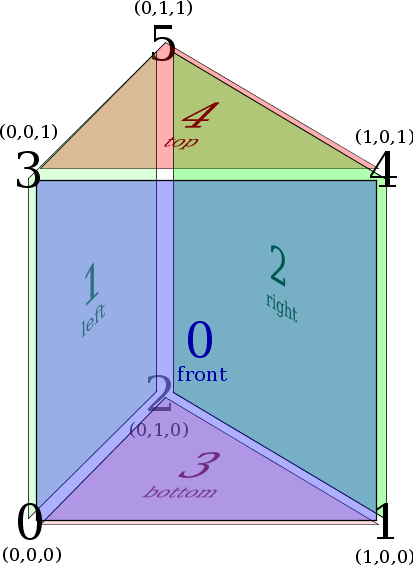
\includegraphics[height=0.23\linewidth]{gg_prism} &
        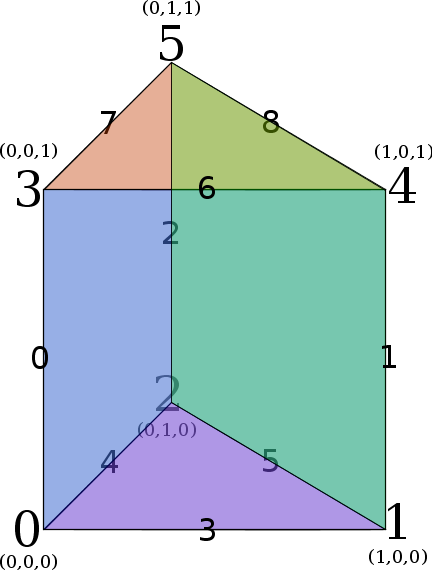
\includegraphics[height=0.23\linewidth]{gg_prism_edges} &
        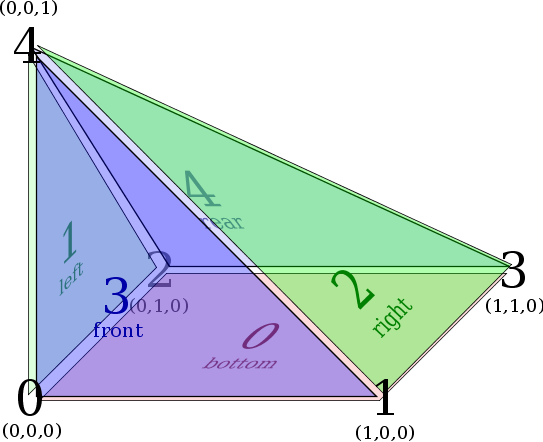
\includegraphics[height=0.23\linewidth]{gg_pyramid} &
        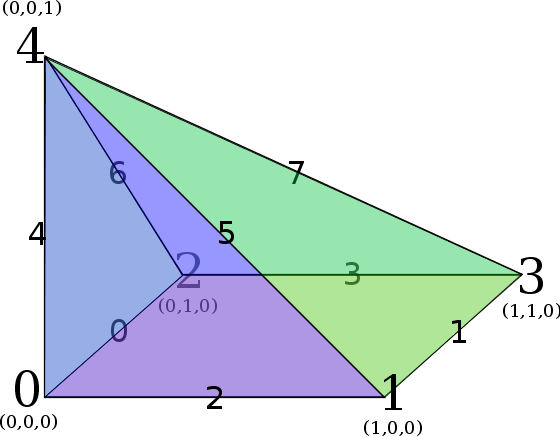
\includegraphics[height=0.23\linewidth]{gg_pyramid_edges}
        \\
        prism (faces) & prism (edges) & pyramid (faces) & pyramid (edges)\\
      \end{tabular}
    \end{center}
  \end{onlyenv}
\end{frame}

\begin{frame}[fragile]
  \frametitle{Geometry Types}
  \lstinline!GeometryType! is a simple identifier for a reference element
  \begin{itemize}
  \item Obtain from entity or geometry object using \lstinline!.type()!
  \item \lstinline!GeometryType! for specific reference elements in namespace \lstinline!Dune::GeometryTypes!:
\begin{cppcode}
namespace GeometryTypes = Dune::GeometryTypes;
Dune::GeometryType gt;

gt = GeometryTypes::vertex;
gt = GeometryTypes::line;
gt = GeometryTypes::triangle;
gt = GeometryTypes::square;
gt = GeometryTypes::hexahedron;
gt = GeometryTypes::cube(dim);
gt = GeometryTypes::simplex(dim);
\end{cppcode}
\item \lstinline!GeometryType!s are cheap, always store and pass around copies (don't use references)
  \end{itemize}

\end{frame}

\begin{frame}[fragile]
  \frametitle{ReferenceElement (I)}
  A reference element provides topological and geometrical information about the embedding of subentities:\\
    ~\hfill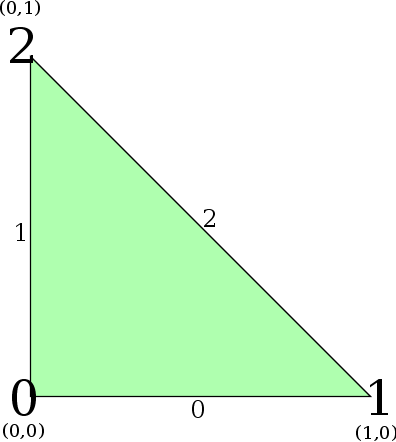
\includegraphics[width=0.24\linewidth]{gg_triangle}
    \hfill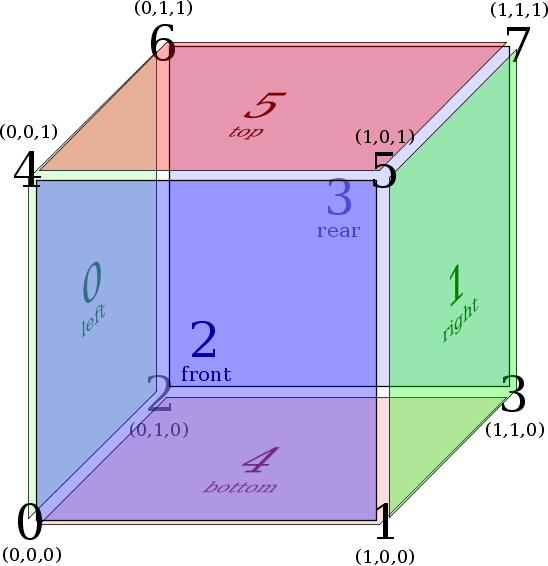
\includegraphics[width=0.28\linewidth]{gg_hexahedron}
    \hfill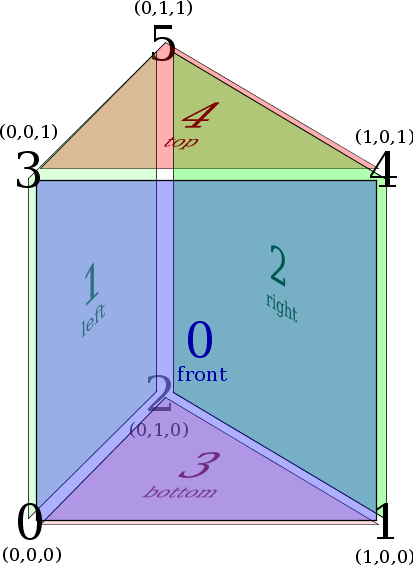
\includegraphics[width=0.22\linewidth]{gg_prism}
    \hfill~

    ~\hfill\parbox{0.24\linewidth}{\centering simplex 2D}
    \hfill\parbox{0.28\linewidth}{\centering cube 3D}
    \hfill\parbox{0.22\linewidth}{\centering prism} \hfill~\\
    \begin{itemize}
    \item Numbering of subentities within the reference element
    \item Geometrical mappings from reference elements of subentities to the current reference element
    \end{itemize}
\end{frame}


\begin{frame}[fragile]
  \frametitle{ReferenceElement (II)}
    \begin{itemize}
    \item Reference elements are templated on the dimension and the coordinate field type
\begin{cppcode}
Dune::ReferenceElement<double,dim> ref_el = ...;
\end{cppcode}
\item The function \lstinline!Dune::referenceElement()! will extract the reference element from most objects
  that have one:
\begin{cppcode}
auto ref_el = Dune::referenceElement(entity.geometry());
\end{cppcode}
    When using this function, you don't have to figure out the template parameters.
    \item \lstinline!ReferenceElement!s are cheap, always store and pass around copies (don't use references)
    \end{itemize}
    For more information see the documentation on reference elements
    (\url{https://dune-project.org/doxygen/master/group__GeometryReferenceElements.html})
\end{frame}


%\only<article>{\newpage}


\subsection{Geometry}

\begin{frame}
  \frametitle{Geometry}

  Transformation $T_E$
  \begin{itemize}
  \item Maps from one space to an other.
  \item Main purpose is to map from the reference element to global coordinates.
  \item Provides transposed inverse of the Jacobian ($J^{-T}(T_E)$).
  \end{itemize}

  \visible<presentation|1->{
    \begin{center}
    \includegraphics[width=0.5\linewidth]{refelem-mapping}\end{center}}


 %  \only<presentation>{\vfill}
 %  \pause
 %  \lstinline!Grid::Codim<c>::Geometry!
 %  provides this data:

 %  \only<presentation>{\vfill}
 %  \pause

 %  \begin{center}
 %    \begin{tabular}{l|l\amode{|p{8cm}}{}}
 %      \hline
 %      Method name & Parameter \amode{& Result}{} \\\hline
 %      \lstinline[basicstyle=\scriptsize\ttfamily]!global! & local coordinate
 %      \amode{& transform from reference (local) coordinate
 %        system to target (global) coordinate system}{}\\
 %      \lstinline[basicstyle=\scriptsize\ttfamily]!local! & global coordinate
 %      \amode{& transform from target (global) coordinate
 %        system to reference (local) coordinate system}{}\\
 %      \lstinline[basicstyle=\scriptsize\ttfamily]!center! & none
 %      \amode{& center of entity in target (global) coordinates}{}\\
 %      \lstinline[basicstyle=\scriptsize\ttfamily]!volume! & none
 %      \amode{& volume of entity in units of the target (global)
 %        coordinate system}{}\\
 %      \lstinline[basicstyle=\scriptsize\ttfamily]!integrationElement! & local coordinate
 %      \amode{& Determinant of the jacobian of the
 %        Transformation from local to global coordinates. For affine
 %        transformations this is the volume}{}\\
 %      \lstinline[basicstyle=\scriptsize\ttfamily]!jacobianInverseTransposed! & local coordinate
 %      \amode{& the inverse of the transposed jacobian of the
 %        transformation; this is necessary to correctly transform
 %        gradients from local to global coordinates}{}
 %      \\\hline
 %    \end{tabular}
 % \end{center}
\end{frame}


\begin{frame}[fragile]
  \frametitle{Geometry Interface (I)}
  \begin{itemize}
  \item Obtain Geometry from entity
    \begin{cppcode}
auto geo = entity.geometry();
    \end{cppcode}
  \item Convert local coordinate to global coordinate
    \begin{cppcode}
auto x_global = geo.global(x_local);
    \end{cppcode}
  \item Convert global coordinate to local coordinate
    \begin{cppcode}
auto x_local = geo.local(x_global);
    \end{cppcode}
  \end{itemize}
\end{frame}


\begin{frame}[fragile]
  \frametitle{Geometry Interface (II)}
  \begin{itemize}
  \item Get center of geometry in global coordinates
    \begin{cppcode}
auto center = geo.center();
    \end{cppcode}
  \item Get number of corners of the geometry (e.g. 3 for a triangle)
    \begin{cppcode}
auto num_corners = geo.corners();
    \end{cppcode}
  \item Get global coordinates of $i$-th geometry corner ($0 \leq i < $\lstinline!geo.corners()!)
    \begin{cppcode}
auto corner_global = geo.corner(i);
    \end{cppcode}
  \end{itemize}
\end{frame}

\begin{frame}[fragile]
  \frametitle{Geometry Interface (III)}
  \begin{itemize}
  \item Get type of reference element
    \begin{cppcode}
auto geometry_type = geo.type(); // square, triangle, ...
    \end{cppcode}
  \item Find out whether geometry is affine
    \begin{cppcode}
if (geo.affine()) {
  // do something optimized
}
    \end{cppcode}
  \item Get volume of geometry in global coordinate system
    \begin{cppcode}
auto volume = geo.volume();
    \end{cppcode}
  \item Get integration element for a local coordinate (required for numerical integration)
    \begin{cppcode}
auto mu = geo.integrationElement(x_local);
    \end{cppcode}
  \end{itemize}
\end{frame}

\begin{frame}[fragile]
  \frametitle{Gradient Transformation}
  Assume
  \begin{equation*}
    f : \Omega \rightarrow \R
  \end{equation*}
 evaluated on a cell $E$, i.e.\ $f\bigl(T_E(\hat{x})\bigr)$.\\[1em] The gradient of $f$ is then given by
 \begin{equation*}
   J_T^{-T}(\hat{x})\hat{\nabla}f\bigl(T_E(\hat{x})\bigr):
 \end{equation*}
  \begin{cppcode}
auto x_global = geo.global(x_local);
auto J_inv = geo.jacobianInverseTransposed(x_local);
auto tmp = gradient(f)(x_global); // gradient(f) supplied by user
auto gradient = tmp;
J_inv.mv(tmp,gradient);
  \end{cppcode}
\end{frame}

\begin{frame}[fragile]
  \frametitle{Obtaining Quadrature Rules}
  Recall: Numerical quadrature rules given by
  \begin{equation*}
    \int_{\hat\Omega} f(x) \diffd x \approx \sum_{i = 1}^N w_i f(x_i)
  \end{equation*}

  \begin{itemize}
  \item \lstinline!dune-geometry! provides pre-defined quadrature rules for common geometry types:
\begin{cppcode}
int order = ...;
Dune::GeometryType gt = ...;
auto& qr = Dune::QuadratureRules<double,dim>::rule(gt,order);
\end{cppcode}
\item The rule factory is parameterized by the number type (typically use \lstinline!Grid::ctype!) and the dimension of the
  integration domain
\item The rule is exact for polynomials up to the given \lstinline!order!
\item Use \lstinline!auto&! for the type of the rule to avoid expensive copies
\item Optional third parameter to select type of rule (Jacobi, Legendre, Lobatto)
  \end{itemize}

\end{frame}

\begin{frame}[fragile]
  \frametitle{Using Quadrature Rules}
  \begin{itemize}
  \item A \lstinline!QuadratureRule! is a range of
    \lstinline!QuadraturePoint!.
  \item \lstinline!QuadraturePoint! provides weight and position:
    \begin{itemize}
    \item \lstinline!QuadraturePoint::weight()!
    \item \lstinline!QuadraturePoint::position()!
    \end{itemize}
  \end{itemize}
  \pause
  \structure{Example}{\footnotesize
\begin{cppcode}
auto f = some_function_to_integrate(...);
double integral = 0.0;
for (const auto& qp : rule)
{
  integral += f(qp.position()) * qp.weight();
}
\end{cppcode}
} \pause \structure{Attention:} When integrating over cells in a grid, keep in mind that the quadrature
point coordinates are local to the reference element and need to be transformed when integrating an analytical function!
\end{frame}

\begin{frame}[fragile]
  \frametitle{Quadrature Rule Access in PDELab}

  Most of the time, you want a quadrature rule for an entity geometry\\[.5em]
  $\Longrightarrow$ no need to specify template types\\[1em]

  PDELab extension to simplify access:
\begin{cppcode}
#include <dune/pdelab/common/quadraturerules.hh>

...

// PDELab quadrature rules wrap dune-geometry rules and are
// cheap to copy, so use "auto" instead of "auto&"
auto quad = Dune::PDELab::quadratureRule(geometry,order);
for (const auto& qp : quad)
{
    auto x_local = qp.position();
    auto w = qp.weight();
}
\end{cppcode}

\end{frame}

% \begin{frame}[fragile]
% \frametitle{Example: Integrating a function u on a GridView}
% \begin{equation*}
% \int_{\Omega}u(x) \diffd x\approx \sum_{E \in GV}\sum_{i \in QR} u(T_e(x_i)) w_i |\det J_E^T(x_i) J_E(x_i)|^{1/2}
% \end{equation*}
% %\begin{cppcode}
% %double value = 0.0, volume = 0.0;
% %for (const auto& cell : elements(gv)) {
% %  auto geo = cell.geometry();
% %  // integrate with numerical quadrature
% %  for (auto& qp : Dune::PDELab::quadratureRule(geo,2)) {
% %    auto x_local = qp.position();
% %    auto x_global = geo.global(x_local);
% %    // accumulate integral contribution
% %    value += f(x_global) *
% %             qp.weight() * geo.integrationElement(x_local);
% %  }
% %  volume += geo.volume();
% %}
% %std::cout << "Average: " << value / volume << std::endl;
% %\end{cppcode}
% \bigskip
% \begin{center}
% Go to code example 2 \ldots
% \end{center}
% \end{frame}

\subsection{Intersections}


\def\intersections{
        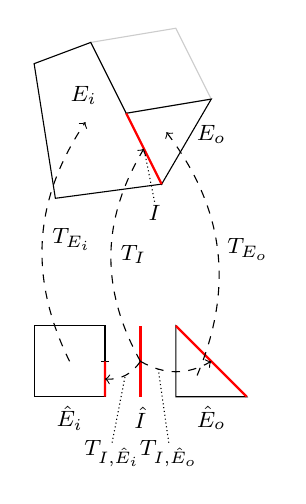
\begin{tikzpicture}[font=\footnotesize,scale=0.9]
\draw(2,0) -- (3,0) -- (2,1) -- cycle;

\draw[thick,red] (1.5,0) -- (1.5,1);

\draw (0,0) rectangle (1,1);

\draw[black!20!white] (1.3,4) -- (2.5,4.2) -- (2,5.2) -- (0.8,5) -- cycle;
\draw (1.8,3) -- (1.3,4) -- (2.5,4.2) -- cycle;
\draw (1.8,3) -- (0.8,5) -- (0,4.7) -- (0.3,2.8) -- cycle;
\draw (0.95,0.5) -- (1.05,0.5);

\draw[thick,red]
  (1,0) -- (1,0.5)
  (2,1) -- (3,0)
  (1.8,3) -- (1.3,4);


\path
  (0.5,0.5) coordinate(e1r)
  (2.3,0.3) coordinate(e2r)
  (1.5,0.5) coordinate(ir)
  (0.725,3.875) coordinate(e1w)
  (1.867,3.733) coordinate(e2w)
  (1.55,3.5) coordinate(iw)
  (1,0.25) coordinate(ie1)
  (2.5,0.5) coordinate(ie2);

\draw[dashed]
  (ir)  edge[->,bend left]  node[right] {$T_I$}       (iw)
  (e1r) edge[->,bend left]  node[right] {$T_{E_i}$}   (e1w)
  (e2r) edge[->,bend right] node[right]  {$T_{E_o}$}   (e2w)
  (ir)  edge[->,bend left]  coordinate(ie1c)  (ie1)
  (ir)  edge[->,bend right] node(ie2c) [near start] {}  (ie2);

\node (ie1label) at(1.1,-0.8) {$T_{I,\hat{E}_i}$};
\node (ie2label) at(1.9,-0.8) {$T_{I,\hat{E}_o}$};
\node (ilabel) at (1.7,2.6) {$I$};

\draw[densely dotted]
  (ie1label)+(0,+1ex) edge (ie1c)
  (ie2label)+(0,+1ex) edge (ie2c.center)
  (ilabel)+(0,+1ex) edge (iw);

\node at(1.5,-0.3) {$\hat{I}$};
\node at(0.5,-0.3) {$\hat{E}_i$};
\node at(2.5,-0.3) {$\hat{E}_o$};
\node at(0.7,4.25) {$E_i$};
\node at(2.5,3.7) {$E_o$};
        \end{tikzpicture}
}

\begin{frame}[fragile]
  \only<presentation>{\frametitle{Intersections}}

  \begin{columns}
    \begin{column}{0.75\linewidth}
      \begin{itemize}
      \item Grids may be non conforming.
      \item Entities can intersect with neighbours and boundary.
      \item Represented by \lstinline!Intersection! objects.
      \item Intersections hold topological and
        geometrical information.
      \item Intersections depend on the view:
      \item \textbf{Note:} Intersections are always of
        codimension 1!
      \end{itemize}
    \end{column}
    \begin{column}{0.25\linewidth}
      \begin{center}
        \intersections{}
      \end{center}
    \end{column}
  \end{columns}

\end{frame}

\begin{frame}[fragile]
  \frametitle{Intersection Interface}
  \begin{itemize}
  \item Is this an intersection with the domain boundary?
    \begin{cppcode}
bool b = intersection.boundary();
    \end{cppcode}
  \item Is there an entity on the outside of the intersection?
    \begin{cppcode}
bool b = intersection.neighbor();
    \end{cppcode}
  \item Get the cell on the inside
    \begin{cppcode}
auto inside_cell = intersection.inside();
    \end{cppcode}
  \item Get the cell on the outside
    \begin{cppcode}
// Do this only if intersection.neighbor() == true
auto outside_cell = intersection.outside();
    \end{cppcode}
  \end{itemize}

\end{frame}



\begin{frame}[fragile] \frametitle{Intersection: Geometries}
  \begin{columns}
    \begin{column}{0.75\linewidth}
      \begin{itemize}
      \item Get mapping from intersection reference element to global coordinates
        \begin{cppcode}
auto world_geo =
    intersection.geometry();
        \end{cppcode}
      \item Get mapping from intersection reference element to reference element of inside cell
        \begin{cppcode}
auto inside_geo =
    intersection.geometryInInside();
        \end{cppcode}
      \item Get mapping from intersection reference element to reference element of outside cell
        \begin{cppcode}
auto outside_geo =
    intersection.geometryInOutside();
        \end{cppcode}
      \end{itemize}
    \end{column}
 \begin{column}{0.25\linewidth}
      \begin{center}
        \intersections{}
      \end{center}
    \end{column}
  \end{columns}

\end{frame}



\begin{frame}[fragile] \frametitle{Intersection: Normals}
  \begin{columns}
    \begin{column}{0.75\linewidth}
      \begin{itemize}
      \item Get unit outer normal for local coordinate.
        \begin{cppcode}
auto unit_outer_normal =
    intersection.unitOuterNormal(x_local);
        \end{cppcode}
      \item Get unit outer normal for center of intersection (good for affine geometries).
        \begin{cppcode}
auto unit_outer_normal =
    intersection.centerUnitOuterNormal();
        \end{cppcode}
      \item Get unit outer normal scaled with integration element (convenient for numerical quadrature).
        \begin{cppcode}
auto integration_outer_normal =
    intersection.integrationOuterNormal(x_local);
        \end{cppcode}
      \end{itemize}
    \end{column}
 \begin{column}{0.25\linewidth}
      \begin{center}
        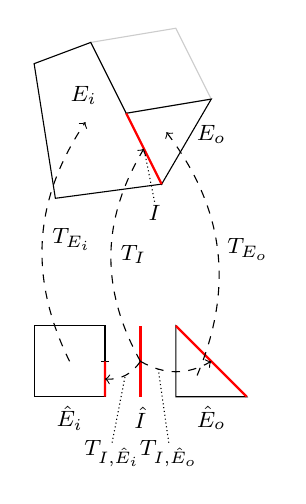
\begin{tikzpicture}[font=\footnotesize,scale=0.9]
\draw(2,0) -- (3,0) -- (2,1) -- cycle;

\draw[thick,red] (1.5,0) -- (1.5,1);

\draw (0,0) rectangle (1,1);

\draw[black!20!white] (1.3,4) -- (2.5,4.2) -- (2,5.2) -- (0.8,5) -- cycle;
\draw (1.8,3) -- (1.3,4) -- (2.5,4.2) -- cycle;
\draw (1.8,3) -- (0.8,5) -- (0,4.7) -- (0.3,2.8) -- cycle;
\draw (0.95,0.5) -- (1.05,0.5);

\draw[thick,red]
  (1,0) -- (1,0.5)
  (2,1) -- (3,0)
  (1.8,3) -- (1.3,4);


\path
  (0.5,0.5) coordinate(e1r)
  (2.3,0.3) coordinate(e2r)
  (1.5,0.5) coordinate(ir)
  (0.725,3.875) coordinate(e1w)
  (1.867,3.733) coordinate(e2w)
  (1.55,3.5) coordinate(iw)
  (1,0.25) coordinate(ie1)
  (2.5,0.5) coordinate(ie2);

\draw[dashed]
  (ir)  edge[->,bend left]  node[right] {$T_I$}       (iw)
  (e1r) edge[->,bend left]  node[right] {$T_{E_i}$}   (e1w)
  (e2r) edge[->,bend right] node[right]  {$T_{E_o}$}   (e2w)
  (ir)  edge[->,bend left]  coordinate(ie1c)  (ie1)
  (ir)  edge[->,bend right] node(ie2c) [near start] {}  (ie2);

\node (ie1label) at(1.1,-0.8) {$T_{I,\hat{E}_i}$};
\node (ie2label) at(1.9,-0.8) {$T_{I,\hat{E}_o}$};
\node (ilabel) at (1.7,2.6) {$I$};

\draw[densely dotted]
  (ie1label)+(0,+1ex) edge (ie1c)
  (ie2label)+(0,+1ex) edge (ie2c.center)
  (ilabel)+(0,+1ex) edge (iw);

\node at(1.5,-0.3) {$\hat{I}$};
\node at(0.5,-0.3) {$\hat{E}_i$};
\node at(2.5,-0.3) {$\hat{E}_o$};
\node at(0.7,4.25) {$E_i$};
\node at(2.5,3.7) {$E_o$};
        \end{tikzpicture}
      \end{center}
    \end{column}
  \end{columns}

\end{frame}



\begin{frame}[fragile] \frametitle{Example: Iterating over intersections}
In order to iterate over the intersections of a given grid cell with respect to some
\lstinline!GridView!, use a range-based for loop with the argument \lstinline!intersections(gv,cell)!.\\[.5em]
The following code iterates over all cells in a \lstinline!GridView! and over all intersections of each cell:
\begin{cppcode}
for (const auto& cell : elements(gv))
  for (const auto& is : intersections(gv,cell)) {
    if (is.boundary()) {
      // handle potential Neumann boundary
    }
    if (is.neighbor()) {
      // code for Discontinuous Galerkin or Finite Volume
    }
  }
\end{cppcode}
\end{frame}

\begin{frame}[fragile] \frametitle{Example: Elementwise divergence of a vector field}
\begin{equation*}
\int_{\Omega_e} \nabla\cdot f(x) \,dx = \int_{\partial \Omega_e} f\cdot n_e \,ds
\end{equation*}
\bigskip
\begin{center}
Go to code example 3 \ldots
\end{center}
\end{frame}

\section{Attaching Data to the Grid}

\begin{frame} \frametitle{Attaching Data to the Grid}

  For computations we need to associate data with grid entities:

  \begin{onlyenv}<1>
  \begin{itemize}
  \item spatially varying parameters,
  \item entries in the solution vector or the stiffness matrix,
  \item polynomial degree for $p$-adaptivity
  \item status information during assembling
  \item \ldots
  \end{itemize}
  \end{onlyenv}

  \begin{onlyenv}<2>
  \begin{itemize}
  \item Allow association of FE computations data with subsets of entities.
  \item Subsets could be ``vertices of level $l$'', ``faces of leaf
    elements'', \ldots
  \item Data should be stored in arrays for efficiency.
  \item Associate index/id with each entity.
  \end{itemize}
  \end{onlyenv}

\end{frame}

\begin{frame}
  \frametitle{Indices and Ids}

  \structure{Index Set:}
  provides a map $m : E \to \mathbb{N}_0$,
  where $E$ is a subset of the entities of a grid view.

  We define the subsets $E_g^c$ of a grid view
  \[ E_g^c = \{e\in E \ | \ \textrm{$e$ has codimension $c$ and geometry type $g$} \}.\]

  \begin{itemize}
  \item unique within the subsets $E_g^c$.
  \item consecutive and zero-starting within the subsets $E_g^c$.
  \item distinct leaf and a level index.
  \end{itemize}

  \pause
  \only<presentation>{\vfill}
  \structure{Id Set:}
  provides a map $m : E \to \mathbb{I}$, where $\mathbb{I}$ is a discrete
  set of ids.

  \begin{itemize}
  \item unique within $E$.
  \item ids need not to be consecutive nor positive.
  \item persistent with respect to grid modifications.
  \end{itemize}

\end{frame}

\begin{frame}[fragile]
  \frametitle{Example: Store the lengths of all edges}
  The following example demonstrates how to
  \begin{itemize}
  \item query an index set for the number of contained
    entities of a certain codimension (so that we can allocate a vector of correct size).
  \item obtain the index of a grid entity from an index set and use it to store associated data.
  \end{itemize}
  \begin{cppcode}
auto& index_set = gv.indexSet();
// Create a vector with one entry for each edge
auto edge_lengths = std::vector<double>(index_set.size(1));
// Loop over all edges and store their length
for (const auto& edge : edges(gv))
  lengths[index_set.index(edge)] = edge.geometry().volume();
\end{cppcode}
\end{frame}

\begin{frame}[fragile]
  \frametitle{Sequential finite volume solver}
Consider the first-order linear PDE
$$ \partial_t u + \nabla\cdot(vu) = 0$$
with given vector field $v(x)$ and unknown solution $u(x,t)$.

The explicit cell-centered finite volume method reads
$$ \bar{u}_e^{k+1} = \bar{u}_e^{k} - \frac{\Delta t}{|\Omega_e|} \sum_{(e,e')\in I(e)}
\Phi(v\cdot n_e,\bar{u}_e^{k},\bar{u}_{e'}^{k}) |I(e,e')|$$
with the numerical flux function $\Phi$ chosen as upwind flux here.

\begin{center}
Go to code example 4 \ldots
\end{center}
\end{frame}

\begin{frame}
  \frametitle{Example: 2D Multi-Element Grid -- Indices}

  \begin{onlyenv}<presentation>
    \structure{Locally refined grid:}
    \vspace*{2ex}
    \begin{overlayarea}{\linewidth}{3ex}
      \medskip
      \begin{onlyenv}<3-6> \emph{Indices:}
      \end{onlyenv}
      \begin{onlyenv}<7-> \emph{Ids:}
      \end{onlyenv}
    \end{overlayarea}
  \end{onlyenv}

  \only<article>{\begin{multicols}{2}}
  \begin{overlayarea}{\linewidth}{0.45\linewidth}
    \begin{center}

    \begin{onlyenv}<1-2>
      \includegraphics[width=0.4\linewidth]{index-grid0}
      \hfill
      \begin{onlyenv}<2>
        \includegraphics[width=0.4\linewidth]{index-grid1}\par
        \only<article>{Locally refined grid\par}
      \end{onlyenv}
    \end{onlyenv}

    \begin{onlyenv}<3>
      \includegraphics[width=0.4\linewidth]{index-vertex0}
      \hfill
      \includegraphics[width=0.4\linewidth]{index-grid1}\par
      Consecutive index for vertices\par
    \end{onlyenv}

    \begin{onlyenv}<4>
      \includegraphics[width=0.4\linewidth]{index-all0}
      \hfill
      \includegraphics[width=0.4\linewidth]{index-grid1}\par
      \ldots{} and cells\par
    \end{onlyenv}

    \begin{onlyenv}<5>
      \includegraphics[width=0.4\linewidth]{index-cell0}
      \hfill
      \includegraphics[width=0.4\linewidth]{index-cell1old}\par
      Old cell indices on refined grid\par
    \end{onlyenv}

    \begin{onlyenv}<6>
      \includegraphics[width=0.4\linewidth]{index-cell0}
      \hfill
      \includegraphics[width=0.4\linewidth]{index-cell1}\par
      Consecutive cell indices on coarse and refined grid\par
    \end{onlyenv}

    \begin{onlyenv}<7>
      \includegraphics[width=0.4\linewidth]{index-id0}
      \hfill
      \includegraphics[width=0.4\linewidth]{index-id1}\par
      Persistent Ids on coarse and refined grid\par
    \end{onlyenv}

    \end{center}
  \end{overlayarea}
  \only<article>{\end{multicols}}
\end{frame}

\begin{frame} \frametitle{Mapper}
  \structure{Mappers extend} the functionality of \structure{Index Sets}.

  \medskip
  \begin{itemize}
  \item associate data with an arbitrary subsets $E'\subseteq E$
    \only<presentation>{\\}
    of the entities $E$ of a grid.
  \item the data $D(E')$ associated with
    $E'$ is stored in an array.
  \item map from the consecutive, zero-starting index $I_{E'} =
    \{0, \ldots, |E'|-1\}$ to the data set $D(E')$.
  \end{itemize}

  \medskip
  Mappers can be easily implemented upon the Index Sets and Id Sets.

  \pause \medskip
  You will be using the

  \centering
  %\footnotesize
  \lstinline!Dune::MultipleCodimMultipleGeomTypeMapper<GridView>!.
\end{frame}

\begin{frame} \frametitle{Example: Mapper (I)}
\scriptsize
\begin{codeblock}
  \lstinputlisting[lastline=16, basicstyle=\scriptsize\ttfamily]{snippets/indizes_cxx11.cc}
\end{codeblock}
\end{frame}

\begin{onlyenv}<presentation>
\begin{frame} \frametitle{Example: Mapper (II)}
\scriptsize
\begin{codeblock}
  \lstinputlisting[firstline=14, basicstyle=\scriptsize\ttfamily]{snippets/indizes_cxx11.cc}
\end{codeblock}
\end{frame}
\end{onlyenv}

\section{Further Reading}

\begin{onlyenv}<presentation>
  \begin{frame}
    \frametitle{Further Reading}
    \only<presentation>{\framesubtitle{What we didn't discuss\dots{}}}
    \begin{itemize}
%    \item grid creation
%      \medskip
%    \item I/O
%      \medskip
    \item grid adaptation
      \medskip
    \item parallelization, load balancing
      \medskip
    \item further specialized methods (e.g. related to grid hierarchy)
    \end{itemize}
  \end{frame}
\end{onlyenv}

\begin{frame} \frametitle<presentation>{Further Reading}
    \only<presentation>{\framesubtitle{Literature}}

    Cite when using the DUNE grid interface\ldots
    \begin{thebibliography}{}

\bibitem[Bastian et al. (2008)]{dune01}
P. Bastian, M. Blatt, A. Dedner, C. Engwer, R. Klöfkorn, M. Ohlberger,
O. Sander.
\newblock A Generic Grid Interface for Parallel and Adaptive
Scientific Computing.
\emph{Part I: Abstract Framework.}
\newblock \emph{Computing,} 82(2--3), 2008, pp.~103--119.

\bibitem[Bastian et al. (2008)]{dune02}
P. Bastian, M. Blatt, A. Dedner, C. Engwer, R. Klöfkorn, M. Ohlberger,
O. Sander.
\newblock A Generic Grid Interface for Parallel and Adaptive
Scientific Computing.
\emph{Part II: Implementation and Tests in DUNE.}
\newblock \emph{Computing,} 82(2--3), 2008, pp.~121--138.

\end{thebibliography}
\end{frame}

\end{document}
